\documentclass[a4paper,11pt]{article}
\usepackage[T1]{fontenc}
\usepackage[utf8]{inputenc}
\usepackage{lmodern}
\usepackage[ngerman]{babel}
\usepackage{cite}
\usepackage{rotating}
\usepackage{graphicx}

\newcommand{\specialcell}[2][c]{%
  \begin{tabular}[#1]{@{}c@{}}#2\end{tabular}}

\title{List of sensor fault detection methods}
\author{Georg Jäger}

\begin{document}

\maketitle


\begin{abstract}
 This document is meant to list up different methods for sensor fault detection. Furthermore, all methods should be classified whether they can handle specific fault types or not. As we assume the sensor signal as the only input of the fault detection methods, another classification is done concerning the dynamic of the input signal. This classification is done by deciding whether a method is able to detect a specific fault type in a high/middle/low dynamic signal. 
\end{abstract}

\tableofcontents
\section{Preparation}
 
\subsection{Fault model}  
  We want to classify sensor fault detection methods concerning specific fault types. The first step is to introduce the underlaying fault model. The model used for this analysis was investigated by Sebastian Zug \cite{Z11}.
  
  
 \begin{figure}[ht]
	\centering
  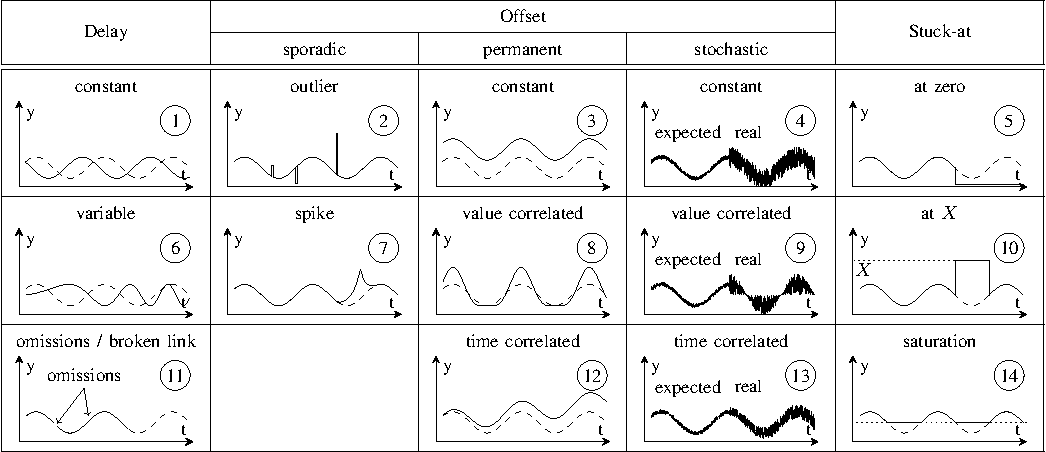
\includegraphics[scale=0.7]{faultmodel.pdf}
	\caption{Faultmodel investigated by Sebastian Zug}
	\label{fig:faultmodel}
\end{figure}



\subsection{Process model}


\section{Methods for sensor fault detection}

Sensor fault detection was addressed by many scientific publications and papers before. Therefore a lot of different approaches are available. As the primary focus of this documentation is on the framework, we only introduce and analyze some before selected data-driven techniques on detecting sensor faults. The input of every detection method is a signal representing the observations of an sensor over time. Beside this, we assume only one-dimensional sensors, e.g distance sensors. As the database will be of the same dimension as the input of the methods, the dimension will be 2 (sensor data and time). 

Furthermore, we want to provide a kind of categorization of this data-driven methods: 
There are three different types of data-driven methods. At first, the fault detection techniques based on pattern recognition. This type of methods analyze the input data in order to find specified patterns, such as fault patterns. Prominent examples of this category are neural networks like \textit{Time-Delay neural networks} and also classifications-methods like nearest-neighbor-classification.

Another type of detection techniques are using time-redundancy for residual or symptom generation. This methods tries to find redundant information in a time-series, such as the average which must be in a certain interval. If this information is deviating from normal values, sensor faults are detected. Examples of this category are \textit{Limit Checking} on the gradient of a signal or an auto-correlation-analysis.

The last type are using models of the underlaying process. By predicting and comparing the sensor observations, they can generate a residual. The process model can be obtained by different approaches. As an example, one could use recurrent neural networks (Elman-networks, NARX) in order to \glqq learn \grqq the model. Another possibility is to determine the transfer function of the system.

\subsection{Detection methods}

\begin{sidewaystable}[h]
 \caption{Summary of all detection methods}
 \begin{tabular}{|c|c|c|c|}
    Name                                & Features                    & Design-Time     & Run-Time   \\  \hline
    1. \textit{Limit Checking}          & \specialcell[c]{Gradient, Average, \\NLPCA-based residual,...} & \specialcell[c]{Find best feature and\\ determine correct threshold} & \specialcell[c]{Calculate feature \\check threshold} \\ \hline
    2. \textit{Adaptive Thresholds}     & \specialcell[c]{Gradient, Average, \\NLPCA-based residual,...} & \specialcell[c]{Find best feature and\\ determing threshold function} & \specialcell[c]{Calculate feature\\ calculate current threshold\\ check threshold } \\ \hline
    3. \textit{Multi-Layer-Perceptron} & Everything is possible & \specialcell[c]{Get Database \\ Determine best features\\ Train MLP} & \specialcell[c]{Calculate feature\\ Determine output of MLP} \\ \hline
    4. \textit{State Observer}          & ODE describing the system   & Determine ODE   & calculate state-space using ODE \\ \hline
    5. \textit{Time-Delay Neural Network} & Everything is possible    & \specialcell[c]{Get Database \\ Determine best features\\ Train NN}   & \specialcell[c]{Calculate features\\ transfer to running window\\ determine output of NN} \\ \hline
    6. \textit{Recurrent Neural Network} & Everything is possible     & \specialcell[c]{Get Database\\ Determine best features\\ Train NN} & \specialcell[c]{Calculate features\\ determine output of NN\\ generate residual by comparing \\output of NN with real sensor data} \\ \hline
    7. \textit{Hidden Markov Model} & Possibilities of every state & \specialcell[c]{Determine relevant states\\ Calculate probabilities of transision} & Update HMM-States \\ \hline
    8. \textit{Wavelet-Analysis}     & - & Determine correct Wavelets  & Wavelet-Analysis needs a convolution \\ \hline
    9. \textit{Fourier-Analysis}    & Calculate running window of signal & \specialcell[c]{determine normal \\frequencies and amplitudes} & online fourier-transformation\\ \hline
    10. \textit{Auto-Correlation-Analysis} & - & \specialcell[c]{determine normal\\ autocorrelation of signal} & requires convolution of signal \\ \hline
 \end{tabular}
 \label{tab:methods}
 \end{sidewaystable}
 
 
 \begin{table}[h]
 \caption{Classification: \glqq Limit-checking of the signals gradient \grqq}
 \begin{tabular}{c|c|c|c}
                    & High dynamic        & Normal dynamic        & Low dynamic \\  \hline
 1. Outlier         & not appropriate     &      OK               &       Well
 \end{tabular}
 \label{tab:lc_gradient}
 \end{table}



\subsection{Recognizing patterns of sensor faults}

Multi-Layer-Perceptron

Time-Delay neural network

Wavelet-Analysis

Hidden-Markov-Models

Support-Vector-Machines

Fuzzy-Classifier

Nearest-Neighbor-Classification 


\subsection{Using time-redundancy for residual/symptom generation}

Gradient-Checking

Average-Checking

Variance-Checking

Auto-correlation-analysis

Fourier-Analysis

Spectrum-Analysis

PCA (AANN)


\subsection{Using process models for residual/symptom generation}
  
MLP's

Recurrent neural network (Elman-Network, NARX)

State-Observer

HMM??

Method of (extended) least squares

Transfer-Functions(DGL)

\bibliography{Literature}{}
\bibliographystyle{plain}


\end{document}
